\section{Sistemas de Coordenadas}

\subsection{Cilíndricas}

\[\Vec{r}(\rho,\phi,z)\]

\begin{figure}[H]
    \centering
    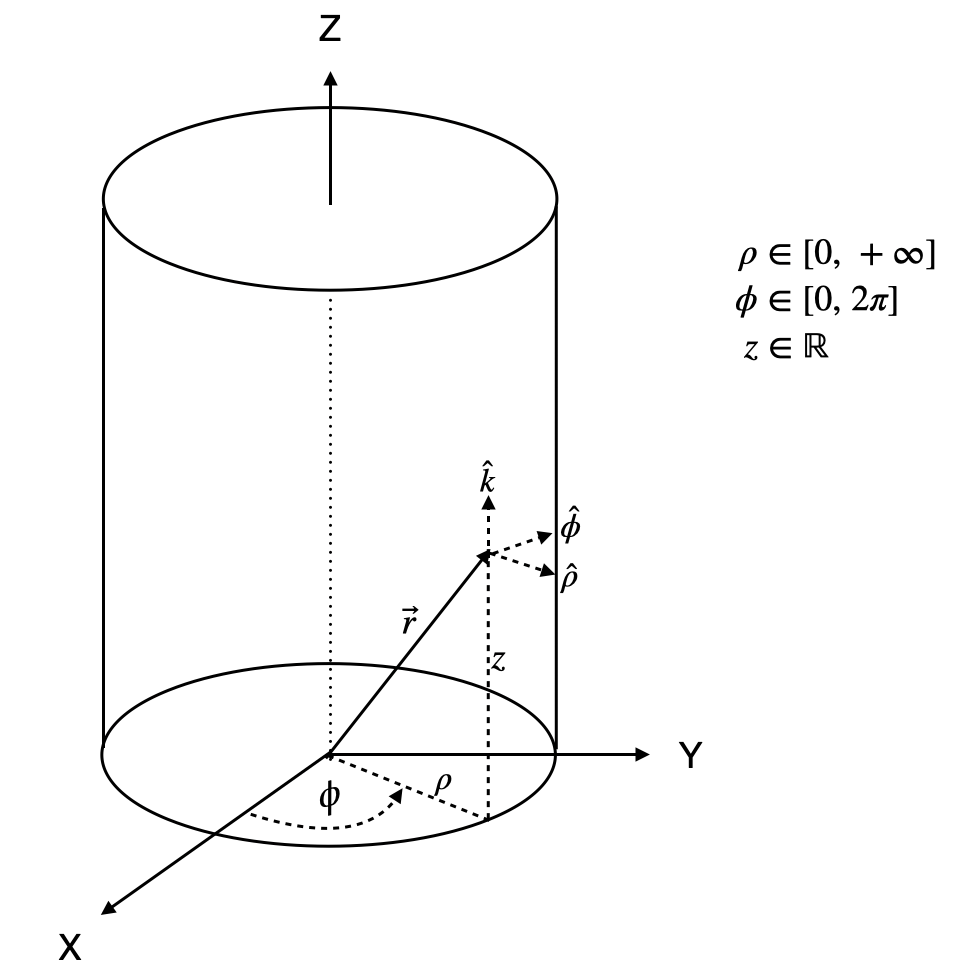
\includegraphics[width=0.45\textwidth]{Resultados Útiles/imgs/coords_cilind_DFI.png}
    \caption{Coordenadas cilíndricas en el plano cartesiano}
    \label{fig:C.cilindricas}
\end{figure}

\begin{minipage}{0.55\textwidth}
\begin{equation}
\begin{split}
    &x = \rho\cos{\phi}\\
    &y = \rho\sin{\phi}\\
\end{split}
\nonumber
\end{equation}
\end{minipage}
\begin{minipage}{0.35\textwidth}
\begin{equation}
\begin{split}
    & \rho = \sqrt{x^2+y^2}\\
    & \phi = \arctan{\frac{y}{x}}\\
\end{split}
\nonumber
\end{equation}
\end{minipage}

\bigbreak
Factores escalares:
\begin{itemize}
    \item $h_\rho = 1$
    \item $h_\phi = \rho$
    \item $h_z = 1$
\end{itemize}

Vectores unitarios:

\begin{itemize}
    \item $\hat{\rho} = \cos{\phi}\,\hat{x}+\sin{\phi}\,\hat{y}$
    \item $\hat{\phi} = -\sin{\phi}\,\hat{x}+\cos{\phi}\,\hat{y}$
    \item $\hat{x}=
    \cos{\phi}\,\hat{\rho}-\sin{\phi}\,\hat{\phi}$
    \item $\hat{y}=
    \sin{\phi}\,\hat{\rho}+\cos{\phi}\,\hat{\phi}$
\end{itemize}

\medbreak

Gradiente:

\[\nabla F = \frac{\partial F}{\partial \rho}\hat{\rho} + \frac{1}{\rho}\frac{\partial F}{\partial \phi}\hat{\phi} + \frac{\partial F}{\partial z}\hat{z}\]

Divergencia:

\[\nabla \cdot \vec{F} = \frac{1}{\rho}\left(\frac{\partial(F_{\rho}\rho)}{\partial\rho}+\frac{\partial F_{\phi}}{\partial\phi}+\frac{\partial(F_{z}\rho)}{\partial z}\right)\]

Rotor:
% Elimine un rho que acompañaba a dF_phi/dphi
\[\nabla\times\vec{F} = \frac{1}{\rho}\left(\frac{\partial F_{z}}{\partial \phi}-\rho\frac{\partial F_{\phi}}{\partial z}\right)\hat{\rho} + \left(\frac{\partial F_{\rho}}{\partial z}-\frac{\partial F_{z}}{\partial \rho}\right)\hat{\phi} + \frac{1}{\rho}\left(\frac{\partial(F_{\phi}\rho)}{\partial \rho}-\frac{\partial F_{\rho}}{\partial \phi}\right)\hat{z}\]

\medbreak

Diferenciales:

\begin{itemize}
    \item Linea:
    \[d\vec{r} = d\rho\hat{\rho} + \rho d\phi\hat{\phi}+dz\hat{z}\]
    \item Superficie:
    \[d\vec{S} = \rho\,d\phi dz\hat{\rho}+d\rho dz\hat{\phi}+\rho\, d\rho d\phi\hat{z}\]
    \item Volumen:
    \[dV = \rho\,d\rho d\phi dz\]
\end{itemize}

\newpage
%%%%%%%%%%%%%%%%%%%%%%%%%%%%%%%%%%%%%%%%%%%%%%%%%%%%%%
\subsection{Esféricas}

\[\Vec{r}(r,\phi,\theta)\]

\begin{figure}[H]
    \centering
    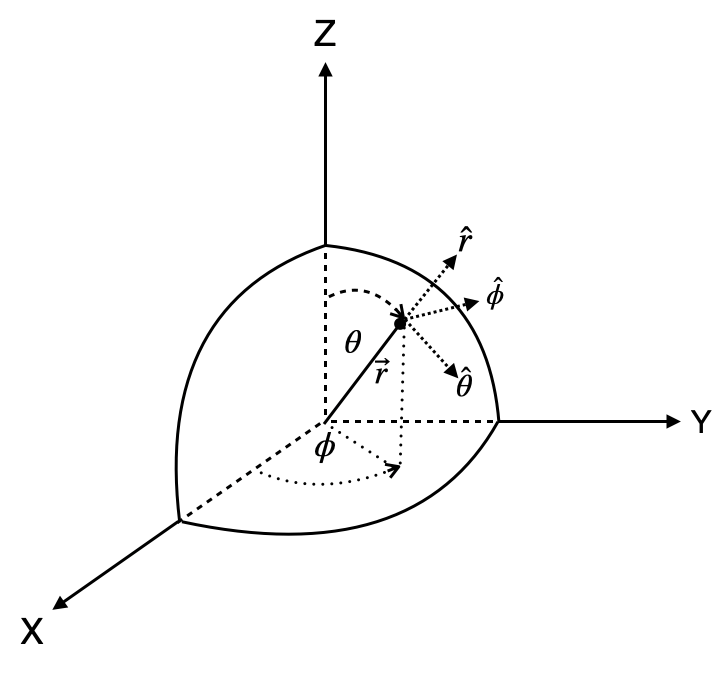
\includegraphics[width=0.5\textwidth]{Resultados Útiles/imgs/coords_esferc_DFI.png}
    \caption{Coordenadas esféricas en el plano cartesiano}
    \label{fig:C.esfericas}
\end{figure}

\begin{minipage}{0.55\textwidth}
\begin{equation}
\begin{split}
    &x = r\sin{\theta}\cos{\phi}\\
    &y = r\sin{\theta}\sin{\phi}\\
    &z = r\cos{\theta}\\
\end{split}
\nonumber
\end{equation}
\end{minipage}
\begin{minipage}{0.35\textwidth}
\begin{equation}
\begin{split}
    & r = \sqrt{x^2+y^2+z^2}\\
    & \phi = \arctan{\frac{y}{x}}\\
    & \theta = \arctan{\left(\frac{\sqrt{x^2+ y^2}}{z}\right)}
\end{split}
\nonumber
\end{equation}
\end{minipage}

\bigbreak
Factores escalares:
\begin{itemize}
    \item $h_r = 1$
    \item $h_\phi = r\sin{\theta}$
    \item $h_\theta = r$
\end{itemize}
\bigbreak
Vectores unitarios:

\begin{itemize}
    \item $\hat{r} = \sin(\theta)\cos(\phi)\hat{x} + \sin(\theta)\sin(\phi)\hat{y} + cos(\theta)\hat{z}$
    \item $\hat{\phi} = -\sin(\phi)\hat{x}+\cos(\phi)\hat{y}$
    \item $\hat{\theta} = \cos(\theta)cos(\phi)\hat{x} + \cos(\theta)\sin(\phi)\hat{y}-\sin(\theta)\hat{z}$
    \item $\hat{x}=\sin{(\theta)\cos{(\phi)}}\hat{r}-\sin{(\phi)}\hat{\phi}+\cos{(\theta)}\cos{(\phi)}\hat{\theta}$
    \item $\hat{y}=\sin{(\theta)\sin{(\phi)}}\hat{r}+\cos{(\phi)}\hat{\phi}+\cos{(\theta)}\sin{(\phi)}\hat{\theta}$
    \item $\hat{z}=\cos{(\theta)}\hat{r}-\sin{(\theta)}\hat{\theta}$
\end{itemize}

\bigbreak

Gradiente:

\[\nabla F = \frac{\partial F}{\partial r}\hat{r} + \frac{1}{rsin(\theta)}\frac{\partial F}{\partial \phi}\hat{\phi} + \frac{1}{r}\frac{\partial F}{\partial \theta}\hat{\theta}\]

Divergencia:

\[\nabla \cdot \vec{F} = \frac{1}{r^2sin(\theta)}\left(\frac{\partial(F_{r}r^2sin(\theta))}{\partial r}+\frac{\partial (F_{\phi}r)}{\partial\phi}+\frac{\partial(F_{\theta}rsin(\theta))}{\partial \theta}\right)\]

Rotor:

\[\nabla\times\vec{F} = \frac{1}{r\sin\theta} \left( \frac{\partial}{\partial \theta} \left(F_\phi\sin\theta \right) - \frac{\partial F_\theta}{\partial \phi} \right) \hat{r} + \frac{1}{r} \left( \frac{1}{\sin\theta} \frac{\partial F_r}{\partial \phi} - \frac{\partial}{\partial r} \left( r F_\phi \right) \right) \hat{\theta} + \frac{1}{r} \left( \frac{\partial}{\partial r} \left( r F_{\theta} \right) - \frac{\partial F_r}{\partial \theta} \right) \hat{\phi}\]

Diferenciales:

\begin{itemize}
    \item Linea:
    \[d\vec{r} = dr\hat{r} + r\sin(\theta)\, d\phi\hat{\phi}+r\,d\theta\hat{\theta}\]
    \item Superficie:
    \[d\vec{S} = r^2\sin(\theta)\,d\phi d\theta\hat{r}+r\,drd\theta\hat{\phi}+r\sin(\theta)\,dr d\phi\hat{\theta}\]
    \item Volumen:
    \[dV = r^2\sin(\theta)\,dr d\phi d\theta\]
\end{itemize}

\newpage
%%%%%%%%%%%%%%%%%%%%%%%%%%%%%%%%%%%%%%%%%%%%%%%%%%%%%%%%%%%%%
\subsection{Parabólicas}

\[\Vec{r}(\epsilon,\eta,\phi)\]

\begin{minipage}{0.55\textwidth}
\begin{equation}
\begin{split}
    &x = \epsilon\eta\cos{\phi}\\
    &y = \epsilon\eta\sin{\phi}\\
    &z = \frac{1}{2}(\eta^2-\epsilon^2)\\
\end{split}
\nonumber
\end{equation}
\end{minipage}
\begin{minipage}{0.35\textwidth}
\begin{equation}
\begin{split}
    & \epsilon = \sqrt{x^2+y^2+z^2}-z\\
    & \eta = \sqrt{x^2+y^2+z^2}+z\\
    & \phi = \arctan{\left(\frac{y}{x}\right)}
\end{split}
\nonumber
\end{equation}
\end{minipage}

\bigbreak
Factores escalares:
\begin{itemize}
    \item $h_\epsilon = \sqrt{\epsilon^2+\eta^2}$
    \item $h_\eta = \sqrt{\epsilon^2+\eta^2}$
    \item $h_\phi = \epsilon\eta$
\end{itemize}
\bigbreak
Vectores unitarios:

\begin{itemize}
    \item $\hat{\epsilon} = \frac{1}{\sqrt{\epsilon^2+\eta^2}}(\eta(\cos{\phi}\,\hat{x}+\sin{\phi}\,\hat{y})-\epsilon\hat{z})$
    \item $\hat{\eta} =  \frac{1}{\sqrt{\epsilon^2+\eta^2}}(\epsilon(\cos{\phi}\,\hat{x}+\sin{\phi}\,\hat{y})+\eta\hat{z})$
    \item $\hat{\phi} = -\sin{\phi}\,\hat{x}+\cos{\phi}\,\hat{y}$
\end{itemize}

\bigbreak

Gradiente:

\[\nabla F = \frac{1}{\sqrt{\epsilon^2+\eta^2}}\frac{\partial
 f}{\partial \epsilon}\hat{\epsilon}+\frac{1}{\sqrt{\epsilon^2+\eta^2}}\frac{\partial
 f}{\partial \eta}\hat{\eta}+\frac{1}{\epsilon\eta}\frac{\partial f}{\partial \phi}\hat{\phi}\]

Divergencia:

\[\nabla \cdot \vec{F} = \frac{1}{\epsilon\eta(\epsilon^2+\eta^2)}
\left(
\frac{\partial(F_\epsilon\epsilon\eta\sqrt{\epsilon^2+\eta^2})}{\partial\epsilon}+
\frac{\partial(F_\eta\epsilon\eta\sqrt{\epsilon^2+\eta^2})}{\partial\eta}+(\epsilon^2+\eta^2)
\frac{\partial F_\phi}{\partial\phi}\right)\]

Rotor:

\[\left(\nabla\times\vec{F}\right)_\epsilon =
\frac{1}{\epsilon\eta\sqrt{\epsilon^2+\eta^2}}
\left(\epsilon
\frac{\partial(F_\phi\eta)}{\partial\eta}-\sqrt{\epsilon^2+\eta^2}\frac{\partial F_\eta}{\partial\phi}\right)\]
\[\left(\nabla\times\vec{F}\right)_\eta=\frac{1}{\epsilon\eta\sqrt{\epsilon^2+\eta^2}}
\left(\sqrt{\epsilon^2+\eta^2}
\frac{\partial F_\epsilon}{\partial\phi}-\eta
\frac{\partial(F_\phi\epsilon)}{\partial\epsilon}\right)\]
\[\left(\nabla\times\vec{F}\right)_\phi=
\frac{1}{\epsilon^2+\eta^2}
\left(\frac{\partial(F_\eta\sqrt{\epsilon^2+\eta^2})}{\partial\epsilon}-\frac{\partial(F_\epsilon\sqrt{\epsilon^2+\eta^2})}{\partial\eta}\right)\]
\newpage
Diferenciales:

\begin{itemize}
    \item Linea:
    \[d\vec{r} = \sqrt{\epsilon^2+\eta^2}d\epsilon\,\hat{\epsilon} + \sqrt{\epsilon^2+\eta^2}d\eta\,\hat{\eta}+\epsilon\eta d\phi\,\hat{\phi}\]
    \item Superficie:
    \[d\vec{S} = \epsilon\eta\sqrt{\epsilon^2+\eta^2}\,d\eta d\phi\hat{\epsilon}+\epsilon\eta\sqrt{\epsilon^2+\eta^2}\,d\phi d\epsilon\hat{\eta}+(\epsilon^2+\eta^2)\,d\epsilon d\eta\hat{\phi}\]
    \item Volumen:
    \[dV = \epsilon\eta(\epsilon^2+\eta^2)\,d\epsilon d\eta d\phi\]
\end{itemize}

\subsection{Elípticas 1}

\[\Vec{r}(\mu,\theta,z)\]

\begin{minipage}{0.55\textwidth}
\begin{equation}
    x = a\cosh{\mu}\cos{\theta}\,\,\,\,\,\,\,\,
    y = a\sinh{\mu}\sin{\theta}
\nonumber
\end{equation}
\end{minipage}

\bigbreak
Factores escalares:
\begin{itemize}
    \item $h_\mu = a\sqrt{\cosh^2{\mu}\cos^2{\theta}
    +\sinh^2{\mu}\sin^2{\theta}}$
    \item $h_\theta = a\sqrt{\cosh^2{\mu}\cos^2{\theta}
    +\sinh^2{\mu}\sin^2{\theta}}$
\end{itemize}
\bigbreak
Vectores unitarios:

\begin{itemize}
    \item $\hat{\mu}=\frac{\sinh{\mu}\cos{\theta}\hat{x}+\cosh{\mu}\sin{\theta}\hat{y}}{\sqrt{\cosh^2{\mu}\cos^2{\theta}
    +\sinh^2{\mu}\sin^2{\theta}}}$
    \item $\hat{\theta}=\frac{-\cosh{\mu}\sin{\theta}\hat{x}+\sinh{\mu}\cos{\theta}\hat{y}}{\sqrt{\cosh^2{\mu}\cos^2{\theta}+\sinh^2{\mu}\sin^2{\theta}}}$
\end{itemize}

\bigbreak

%Gradiente:



%Divergencia:



%Rotor:



%Diferenciales:

%\begin{itemize}
%    \item Linea:
    
%    \item Superficie:
    
%    \item Volumen:
    
%\end{itemize}

\newpage